% !TEX program = tectonic
\documentclass[9pt,a4paper]{article}

\usepackage[left=0.82cm,right=0.82cm,top=0.66cm,bottom=0.62cm]{geometry}
\usepackage{fontspec}
\usepackage{xeCJK}
\usepackage{graphicx}
\usepackage{tabularx}
\usepackage{array}
\usepackage{enumitem}
\usepackage{titlesec}
\usepackage[hidelinks]{hyperref}
\usepackage{xcolor}

\IfFontExistsTF{Arial}{\setmainfont{Arial}}{\setmainfont{TeX Gyre Heros}}
\IfFontExistsTF{Microsoft YaHei}
  {\setCJKmainfont[BoldFont=Microsoft YaHei Bold]{Microsoft YaHei}}
  {\setCJKmainfont[BoldFont=SimHei]{SimSun}}

\setlength{\parindent}{0pt}
\setlength{\tabcolsep}{0pt}
\setlength{\emergencystretch}{1.5em}
\XeTeXlinebreaklocale "zh"
\XeTeXlinebreakskip=0pt plus 0.85pt
\pagenumbering{gobble}
\raggedbottom
\urlstyle{same}

\definecolor{textgray}{HTML}{575757}
\definecolor{rulegray}{HTML}{AEB4BC}

\titleformat{\section}
  {\fontsize{13.1}{15.1}\selectfont\bfseries}
  {}{0pt}{}
  [\vspace{0.07em}{\color{rulegray}\titlerule[0.45pt]}]
\titlespacing*{\section}{0pt}{0.48em}{0.30em}

\setlist[itemize]{
  leftmargin=1.58em,
  labelsep=0.42em,
  itemsep=0.20em,
  topsep=0.15em,
  parsep=0pt,
  partopsep=0pt,
  after=\vspace{0.22em},
  label=\raisebox{0.18ex}{\tiny$\bullet$}
}

\newcommand{\entryheading}[3]{%
  \begin{tabularx}{\textwidth}{@{}X r@{}}
    {\fontsize{10.4}{12.4}\selectfont\textbf{#1}}\hspace{0.48em}{\fontsize{9.55}{11.6}\selectfont\color{textgray}#2} &
    {\fontsize{9.45}{11.4}\selectfont\color{textgray}#3} \\
  \end{tabularx}\vspace{0.09em}
}

\newcommand{\eduheading}[4]{%
  \begin{tabularx}{\textwidth}{@{}X r@{}}
    {\fontsize{10.1}{12.0}\selectfont\textbf{#1}}\hspace{0.45em}{\fontsize{9.35}{11.3}\selectfont\color{textgray}#2} &
    {\fontsize{9.3}{11.2}\selectfont\color{textgray}#3} \\[0.04em]
    {\fontsize{9.25}{11.2}\selectfont #4} & \\
  \end{tabularx}\vspace{0.14em}
}

\newcommand{\projectname}[1]{%
  {\fontsize{9.9}{11.9}\selectfont\textbf{#1}}\par\vspace{0.06em}
}

\newcommand{\tagitem}[2]{\item \textbf{#1：}#2}
\newcommand{\internshipgap}{\vspace{0.16em}}

\begin{document}
\fontsize{9.75}{12.75}\selectfont

\begin{tabularx}{\textwidth}{@{}X >{\raggedleft\arraybackslash}p{2.30cm}@{}}
  \begin{minipage}[t]{\linewidth}
    {\fontsize{23.5}{25.5}\selectfont\bfseries 管振凯}\\[0.34em]
    {\fontsize{10.0}{11.8}\selectfont 男 · 24岁 \enspace|\enspace 意向岗位：AI 产品经理}\\[0.28em]
    {\fontsize{9.0}{10.8}\selectfont
      TEL / WeChat：177\,6812\,0084 \enspace|\enspace
      E-mail：\href{mailto:522024140056@smail.nju.edu.cn}{522024140056@smail.nju.edu.cn}
    }\\[0.12em]
    {\fontsize{9.0}{10.8}\selectfont
      作品集：\href{https://raddddder.github.io/portfolio/}{\underline{raddddder.github.io/portfolio}}
    }
  \end{minipage}
  &
  \raisebox{-0.84\height}{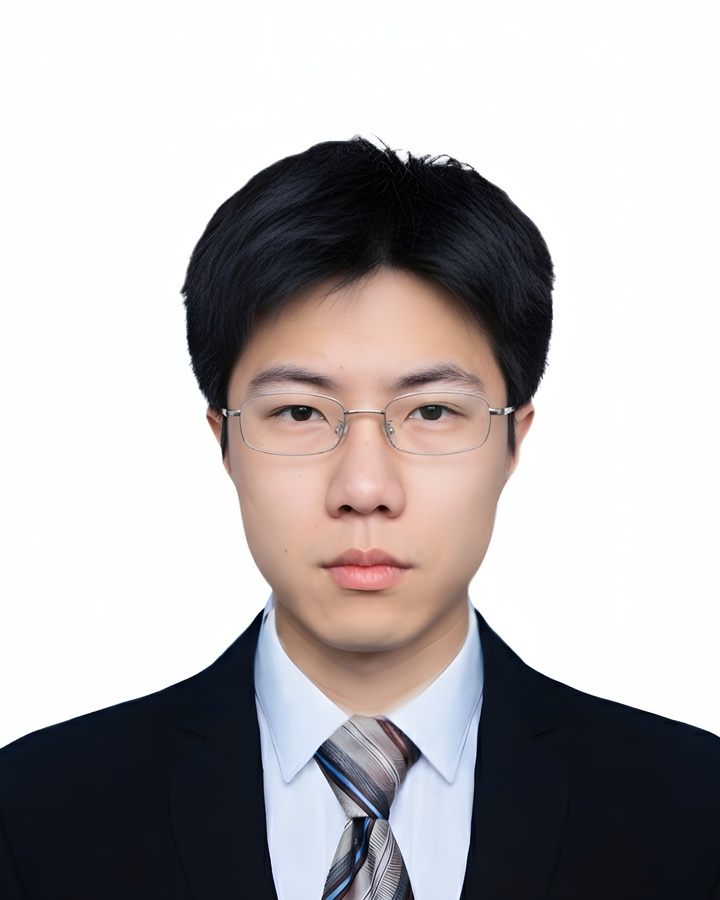
\includegraphics[width=2.08cm,height=2.61cm]{resume-photo.jpg}}
\end{tabularx}

\vspace{-0.24em}
\section{教育背景}

\eduheading
  {南京大学}
  {信息管理学院 · 图书情报硕士}
  {2024.09 -- 2027.06}
  {学业一等奖；2025 贝恩杯案例大赛 12 强}

\eduheading
  {南京邮电大学}
  {计算机学院 · 计算机科学与技术学士}
  {2020.09 -- 2024.06}
  {国家级大学生创新创业训练项目；国家发明专利已授权（第一发明人，\href{https://patents.google.com/patent/CN116453224B/zh}{\underline{CN116453224B}}）；CET-6}

\vspace{-0.10em}
\section{实习经历}

\entryheading{腾讯互动娱乐 IEG · K6 合作部}{产品策划}{2026.06 -- 2026.08}
\projectname{负责项目：英雄联盟攻略服务}
\begin{itemize}
  \tagitem{核心痛点}{面向英雄联盟峡谷玩家，结合 WeGame 备战日均 620 万 PV、用户反馈与对战数据，梳理从一键配置到进阶分析的分层攻略需求；聚焦\textbf{国服数据口径不一致、内容更新慢与入口分散}的问题，建立统一、可信、跨端复用的攻略服务。}
  \tagitem{方案落地}{负责掌盟移动端与数据站 PC 端同步建设，重点落地\textbf{异常对局清洗、榜单算法迭代与场景化数据聚合}，上线英雄/版本榜单、英雄梯度、出装/符文及对线查询；设计“大数据挖掘 -- AI 解读 -- 多端分发”链路，提升版本响应速度。}
  \tagitem{业务结果}{\textbf{数据服务 DAU 达 10 万+}；榜单与英雄梯度攻略在版本更新当日\textbf{由 1.1 万提升至 1.8 万，增长约 64\%}，验证官方国服数据与版本同步攻略能够显著提升玩家回访和攻略消费。}
  \tagitem{AI 助手}{规划掌盟 AI 助手作为\textbf{攻略服务的统一交互入口}，承接局前备战、局中辅助与局后复盘，逐步串联社交、账号资产、战绩、赛事等一站式服务；设计虚拟形象、状态动作、用户画像与长期记忆，提供个性化陪伴。}
\end{itemize}
\internshipgap

\entryheading{京东科技 · 人工智能业务部}{AI 产品经理}{2026.04 -- 2026.06}
\projectname{负责产品：JoyPM｜产品经理数字员工}
\begin{itemize}
  \tagitem{产品定义}{针对产品经理从需求构想到 PRD/方案初稿耗时 \textbf{4--6 小时}、历史方案复用困难与评审返工频繁的问题，0--1 负责 JoyPM 产品经理数字员工，明确\textbf{知识检索辅助、方案生成和质量评测}三类核心产品能力。}
  \tagitem{方案设计}{搭建\textbf{“知识召回 -- 方案生成 -- 自动评测 -- 优质内容回流”}闭环，设计角色知识库与 Agent 工作流，引入人工复核机制，使 AI 产出\textbf{可引用、可审核、可修订}并持续回流知识库。}
  \tagitem{业务结果}{需求到可评审初稿的周期缩短至 \textbf{45 分钟以内}，评测耗时降低 \textbf{30\%}；沉淀标准化角色知识库与 Agent 工作流，形成“方案生成 -- 自动评测 -- 优质内容回流”的\textbf{可复用产品闭环}，为后续同类场景快速迁移提供基础。}
\end{itemize}
\internshipgap

\entryheading{腾讯金融科技 FIT}{AI 产品经理}{2025.09 -- 2026.03}
\projectname{负责产品：Sia｜AI 访谈与调研系统}
\begin{itemize}
  \tagitem{产品定义}{针对传统访谈招募成本高、样本有限、洞察慢且结论难溯源的问题，负责 Sia 的产品设计与研发落地，将人工访谈重构为\textbf{可配置、可追问、可溯源}的 AI 调研产品。}
  \tagitem{核心机制}{搭建\textbf{“大纲配置 -- AI 主持追问 -- 洞察生成 -- 原文溯源”}流程，设计访谈路径控制、动态追问、回答澄清、偏题拉回、策略自适应与证据绑定机制，兼顾\textbf{访谈深度与结论可信度}。}
  \tagitem{业务结果}{覆盖 \textbf{500+ 样本、3 个部门}；项目周期从 \textbf{7 天缩短至 8 小时}，人力成本降低 \textbf{50\%}，获 FIT AI 创新奖。}
\end{itemize}
\internshipgap

\entryheading{波士顿咨询公司 BCG}{项目助理}{2025.06 -- 2026.03}
参与制造业 AI 转型与商业分析，设计 \textbf{2 套面向 CAD 的多模态 Agent 工作流}，将重复操作成本降低约 \textbf{80\%}。\par\vspace{0.22em}

\entryheading{上海人工智能实验室}{战略与 AI 应用实习生}{2025.01 -- 2025.07}
参与 Migo AI 学研助手，主导 QuestPaper 交互原型并协同上线；开展政策与产业研究，完成 \textbf{10+ 篇}专题报告。\par\vspace{0.16em}

\section{AI 项目}
\entryheading{WorkOS｜个人工作记忆系统}{个人项目}{}
\begin{itemize}
  \tagitem{痛点挖掘}{针对工作信息分散、任务进展与判断依据难以回溯的问题，定义可追溯、隐私优先的个人工作记忆产品。}
  \tagitem{方案设计}{独立完成本地优先桌面端 MVP，将屏幕、剪贴板与白板记录聚合为连续工作事件，支持时间线与来源反查。}
  \tagitem{AI 功能}{以多模态模型提取任务、进度及实体关系，生成每日总结与带来源问答；只读 AI 不执行写入或自动操作。}
\end{itemize}

\section{自我评价}
\begin{itemize}
  \tagitem{用户洞察}{善于从用户行为、反馈与具体场景中识别真实需求，将模糊痛点转化为可验证的产品机会。}
  \tagitem{策划与协同}{围绕目标整合数据、技术、内容与业务资源，协调各方形成共识，推动方案落地并取得结果。}
  \tagitem{动手实践}{热衷将好玩的点子做成可用产品，主动学习并补齐所需技能；对 AGI 的到来感到兴奋，持续探索 AI 原生产品。}
\end{itemize}

\section{其他}
\begin{itemize}
  \tagitem{技能}{Codex 等 AI 原生工具包；Figma；XMind；Office 套件。}
  \tagitem{兴趣爱好}{参加电影节、逛博物馆、看演出、旅游。}
\end{itemize}

\end{document}
